\documentclass[crop, tikz]{standalone}
\usepackage{tikz}

% Colour
\usepackage{xcolor}
\colorlet{LightCyan}{cyan!30}
\colorlet{LightGray}{lightgray!30}

% Nodes
\tikzstyle{LSTMblock}=[draw,fill=LightCyan,minimum size=20pt,inner sep=1pt]
\tikzstyle{ConcatBlock}=[draw,fill=LightGray,minimum size=20pt,inner sep=1pt]
\tikzstyle{invisNode}=[circle, line width=0mm, minimum size=20pt, inner sep=0pt]
\tikzstyle{stateTransition}=[-stealth, thick]
% Reverse direction vector arrow
\usepackage{graphicx}
\newcommand{\cev}[1]{\reflectbox{\ensuremath{\vec{\reflectbox{\ensuremath{#1}}}}}}

\begin{document}
    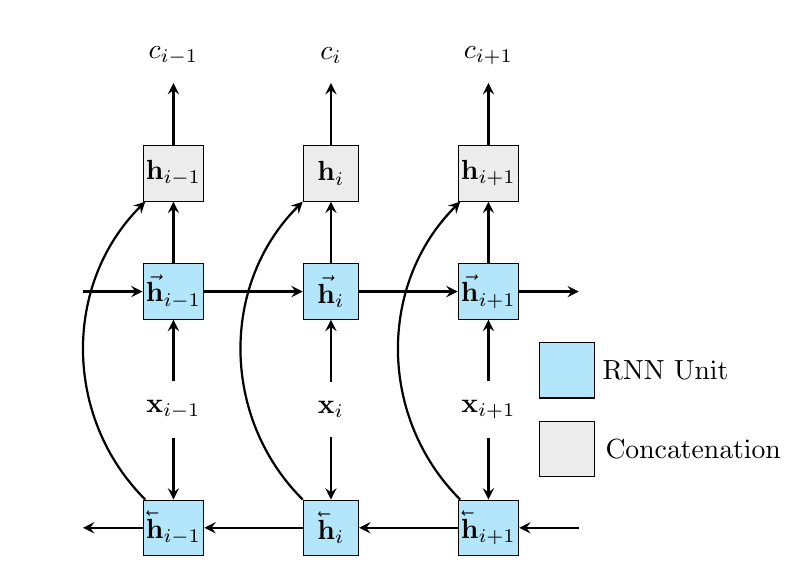
\begin{tikzpicture}
        % Confidence
        \node[invisNode] (y0) at (-2, 3) {$c_{i-1}$};
        \node[invisNode] (y1) at (0, 3) {$c_{i}$};
        \node[invisNode] (y2) at (2, 3) {$c_{i+1}$};
    
        % Concat    
    	\node[ConcatBlock] (c0) at (-2, 1.5) {$\mathbf{h}_{i-1}$};
    	\node[ConcatBlock] (c1) at (0, 1.5) {$\mathbf{h}_{i}$};
    	\node[ConcatBlock] (c2) at (2, 1.5) {$\mathbf{h}_{i+1}$};
    	
    	% Concat -> Confidence
    	\draw[stateTransition] (c0) to[out=90,in=270] node [midway, sloped, above] {} (y0);
    	\draw[stateTransition] (c1) to[out=90,in=270] node [midway, sloped, above] {} (y1);
    	\draw[stateTransition] (c2) to[out=90,in=270] node [midway, sloped, above] {} (y2);

        % Features / input
        \node[invisNode] (x0) at (-2, -1.5) {$\mathbf{x}_{i-1}$};
        \node[invisNode] (x1) at (0, -1.5) {$\mathbf{x}_{i}$};
        \node[invisNode] (x2) at (2, -1.5) {$\mathbf{x}_{i+1}$};

        % Forward Direction
        \node[LSTMblock] (h0) at (-2, 0) {$\vec{\mathbf{h}}_{i-1}$};
        \node[LSTMblock] (h1) at (0, 0) {$\vec{\mathbf{h}}_{i}$};
        \node[LSTMblock] (h2) at (2, 0) {$\vec{\mathbf{h}}_{i+1}$};
        \node[invisNode] (i0) at (-3.5, 0) {};
        \node[invisNode] (i1) at (3.5, 0) {};

    	\draw[stateTransition] (i0) to[out=0,in=180] node [midway, sloped, above] {} (h0);
    	\draw[stateTransition] (h0) to[out=0,in=180] node [midway, sloped, above] {} (h1);
    	\draw[stateTransition] (h1) to[out=0,in=180] node [midway, sloped, above] {} (h2);
    	\draw[stateTransition] (h2) to[out=0,in=180] node [midway, sloped, above] {} (i1);

    	\draw[stateTransition] (x0) to[out=90,in=270] node [midway, sloped, above] {} (h0);
    	\draw[stateTransition] (x1) to[out=90,in=270] node [midway, sloped, above] {} (h1);
    	\draw[stateTransition] (x2) to[out=90,in=270] node [midway, sloped, above] {} (h2);
    	
    	\draw[stateTransition] (h0) to[out=90,in=270] node [midway, sloped, above] {} (c0);
    	\draw[stateTransition] (h1) to[out=90,in=270] node [midway, sloped, above] {} (c1);
    	\draw[stateTransition] (h2) to[out=90,in=270] node [midway, sloped, above] {} (c2);
    	
    	% Backwards direction
        \node[LSTMblock] (h3) at (-2, -3) {$\cev{\mathbf{h}}_{i-1}$};
        \node[LSTMblock] (h4) at (0, -3) {$\cev{\mathbf{h}}_{i}$};
        \node[LSTMblock] (h5) at (2, -3) {$\cev{\mathbf{h}}_{i+1}$};
        \node[invisNode] (i2) at (-3.5, -3) {};
        \node[invisNode] (i3) at (3.5, -3) {};

    	\draw[stateTransition] (h3) to[out=180,in=0] node [midway, sloped, above] {} (i2);
    	\draw[stateTransition] (h4) to[out=180,in=0] node [midway, sloped, above] {} (h3);
    	\draw[stateTransition] (h5) to[out=180,in=0] node [midway, sloped, above] {} (h4);
    	\draw[stateTransition] (i3) to[out=180,in=0] node [midway, sloped, above] {} (h5);
    	
    	\draw[stateTransition] (x0) to[out=270,in=90] node [midway, sloped, above] {} (h3);
    	\draw[stateTransition] (x1) to[out=270,in=90] node [midway, sloped, above] {} (h4);
    	\draw[stateTransition] (x2) to[out=270,in=90] node [midway, sloped, above] {} (h5);
    	
    	\draw[stateTransition] (h3) to[out=135,in=225] node [midway, sloped, above] {} (c0);
    	\draw[stateTransition] (h4) to[out=135,in=225] node [midway, sloped, above] {} (c1);
    	\draw[stateTransition] (h5) to[out=135,in=225] node [midway, sloped, above] {} (c2);
    	
    	\node[LSTMblock] (LSTMLegend) at (3, -1) {};
        \node[invisNode] (LSTMtext) at (4.25,-1) {RNN Unit};
        \node[ConcatBlock] (concatLegend) at (3,-2) {};
        \node[invisNode] (LSTMtext) at (4.6,-2) {Concatenation};

    \end{tikzpicture}

\end{document}